{\color{indiagreen}\subsection{Lokacija in tipi datotek}}
Unity pokriva velik spekter različnih formatov iz različnih programov, kot so npr. Blender, Maya, Photoshop itd. Vsi datote se nahajajo v Asset mapi, ki je potem tudi vidna v samem Unity editorju. V spodnji sliki lahko tudi vidimo tipično strukturo map, ko se naredi nov Unity projekt.\\
\begin{figure}[ht!]
	\centering
	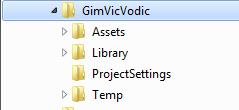
\includegraphics[width=5cm, height=5cm,keepaspectratio=true]{Importing1.png}
	\caption{Struktura map}
\end{figure}
Pri tipičnih formatih datotek kot so npr. JPG, PSD, PNG, MA, BLED, FBX, WAW itd. lahko datoteko, kar kopiramo v asset mapo ali jo celo povlečemo v prav specifično mapo kjer hočemo in se bo prikazala v Unity urejevalniku. Takole so potem urejene datoteke v samem unity-ju.\\
\begin{figure}[ht!]
	\centering
	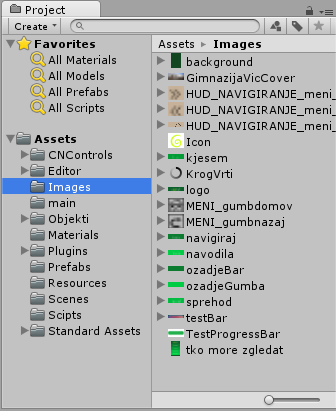
\includegraphics[width=6cm, height=6cm,keepaspectratio=true]{Importing2.png}
	\caption{Pregled map v unity-ju}
\end{figure}
Ko mi kopiramo datoteko v asset mapo, unity poskrbi, da glede na končnico oz. tip se pravilno vključi, compresira in nakoncu postane tudi presentativna v urejevalniku. Pri tem lahko tudi sami spreminjamo določene parametre:
\begin{itemize}
	\item kakšnega tipa je datoteka(sprite, textura, normal map itd.)
	\item kako gosto naj bojo piksli(če je slika)
	\item kaliko prostora lahko zasede na disku
	\item kako naj se kompresira
\end{itemize}
Nakoncu je ponujena možnost, da za različno platformo(Android, IOS, PC, PS3) različno nastavimo import nastavitve. Spodaj lahko na primeru vidimo kaksšne opcije so namna voljo.
\begin{figure}[ht!]
	\centering
	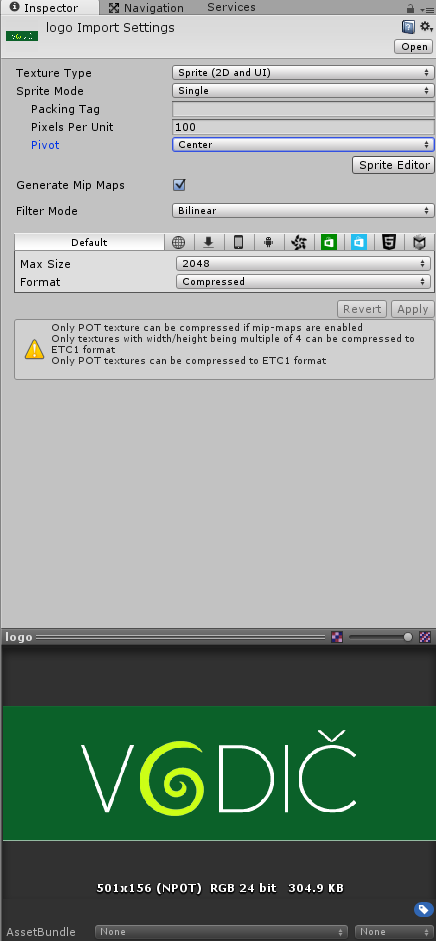
\includegraphics[width=5cm, height=9cm,keepaspectratio=true]{Importing3.png}
	\caption{Import nastavitve}
\end{figure}